%!TEX root = ../thesis.tex
%*******************************************************************************
%****************************** Second Chapter *********************************
%*******************************************************************************

\chapter{The Rotating Sun}

\section{Differential Rotation}
The sun is known to rotate, unlike the earth, differentially. This means that angular rate of rotation of a point in the sun about its spin axis is depends on depth and latitude, $\Omega = \Omega(r,\theta)$. Splitting of p-mode frequencies due to differential rotationis well understood\cite{ritzwoller} and has a long history of inversion analysis\cite{schou98}.
This $\Omega$ is generally taken to be symmetric about the equitorial plane because the antisymmtric part of $\Omega$ is found to leave no signature in the acoustic frequency spcectrum in the first order as a result of a selection rule that arises from perturbation theory; this will be shown at the end of this chapter.

As a result of Alfven's freezing theorem, differential rotation is responsible for winding the solar magnetic field around its spin axis in an axis symmtric fashion. (refer something on this); thus for the most part we'll be investigating the effects of an axis symmetric magnetic field on the spectrum in this work.

\section{Detection from frequency spectrum}

Because of axis symmetry of differential rotation, the flow profile is given as,

\begin{equation}
\vrot = \sum_{s = 1,3,5,...}^{\infty} -w_s^0(r) \partial_{\theta} Y_s^0 \ev{\phi}
\end{equation}

Note that $w_1^0$ is responsible for shell like (pure) rotation as it couples with $\partial_{\theta} Y_1^0 \propto \sin\theta$. Hence $w_3^0$ onwards components of flow are responsible for the differential part of the rotation. Finding frequency splittings due to differential rotatioin is a problem in degenrate perturbation (dpt) or quasi-degenerate perturbation theory depending on whether we're using the isolated multiplet assumption or not. Below we outline the qdpt approach to the problem because when applied to a single multiplet $_n S_l$ it reduces to the dpt approach; \cite{lavely92} contains a more detailed discussion on this topic; it, however, argues via analysis of \mode{n}{1} and \mode{n}{3} multiplets that eigenfrequency correction due to mode-mixing between these two is negligible ($\sim 0.1 \mu Hz$). I'll show in this work that for higher frequency modes with $l\sim 100$ a frequency correction close to $0.4 \mu Hz$ is obtained when qdpt is used, which is close to the correction obtained due presence of realistically strong magnetic fields too, and hence cannot be ignored in an analysis which accounts for both differential rotation and magnetic fields.

\subsection{QDPT Analysis}
The pertubation operator \dLd for a differential rotaional flow is given by 
\begin{equation}
\dLd = -2i \omega \rho \vrot \cdot \grad
\end{equation}
where $\omega$ is the reference frequency in the problem, and $\rho$ is the static background density profile.
The supermatrix element $Z_{k' k}$ for a pertubation \dLd is given by
\begin{equation}
Z_{k' k} = \Lamdr_{k'k} - \delta_{k'k} (\omref^2 - \omega_k^2)
\end{equation}
where $\Lamdr$ is the coupling matrix element $\Lamdr = \inner{\xiv_{k'}}{\dLd \xiv_{k}}$ .
Coupling matrix element is given by
\begin{equation}
\Lamdr_{k'k} = 8 \pi \omref \gam{l'}\gam{l} \oddsum{s} \gam{s} \wigred{-m}{0}{m} \ints dr 
r^2 w_s^0(r) T_s(r)
\end{equation}
where the sensitivity kernel $T_s$ is given by
\begin{dmath}
T_s(r) = (1-(-1)^{s+l+l'}) \om{l'}{0} \om{l}{0} \wigred{-1}{0}{1} r^{-1}
 \enc{U'V+V'U-U'U-\frac{1}{2}\enc{l'(l'+1) + l(l+1) - s(s+1) V'V}}
\end{dmath}
where the rounded brackets represent Wigner 3j symbols. 
\subsection{Selecition rules in mode coupling}\label{sec:selec_rules}
This matrix element enforces the following selection rules for inter-mode interaction which derive from the properties of Wigner 3j symbols \cite{lavely92}.
\begin{enumerate}
\item $m'=m$
\item $l'+l+s = \text{odd}$
\item $|l'-l| \leq s \leq l'+l$
\end{enumerate}
It should be noted here that even though only sum over odd s is considered, the expression for $T_s$ is general and holds for all $s$. This has been verified independently using the Mathematica packaged developed for the sake of this work. This means as far as self coupling is concerned ($l'=l$), the matrix element vanish for all even s.

\subsubsection{Form of supermatrix $Z_{k'k}$}

It is clear from selection rule (1) in \ref{sec:selec_rules} that $Z_{k'k}$ is going to be a sparse matrix consisting of a diagonal and a number of sub-diagonals (proportional to number of multiplets being considered). Also, as $s$ is always odd, $l-l'$ has to be even for non-zero coupling as consequence of selection rule (2). This influences our choice of modes whose inter-coupling will be studied hereafter. Figure (\ref{fig:coup_mat}) is a visual representation of a typical supermatrix consisting of three multiplets.

\begin{figure}[h]
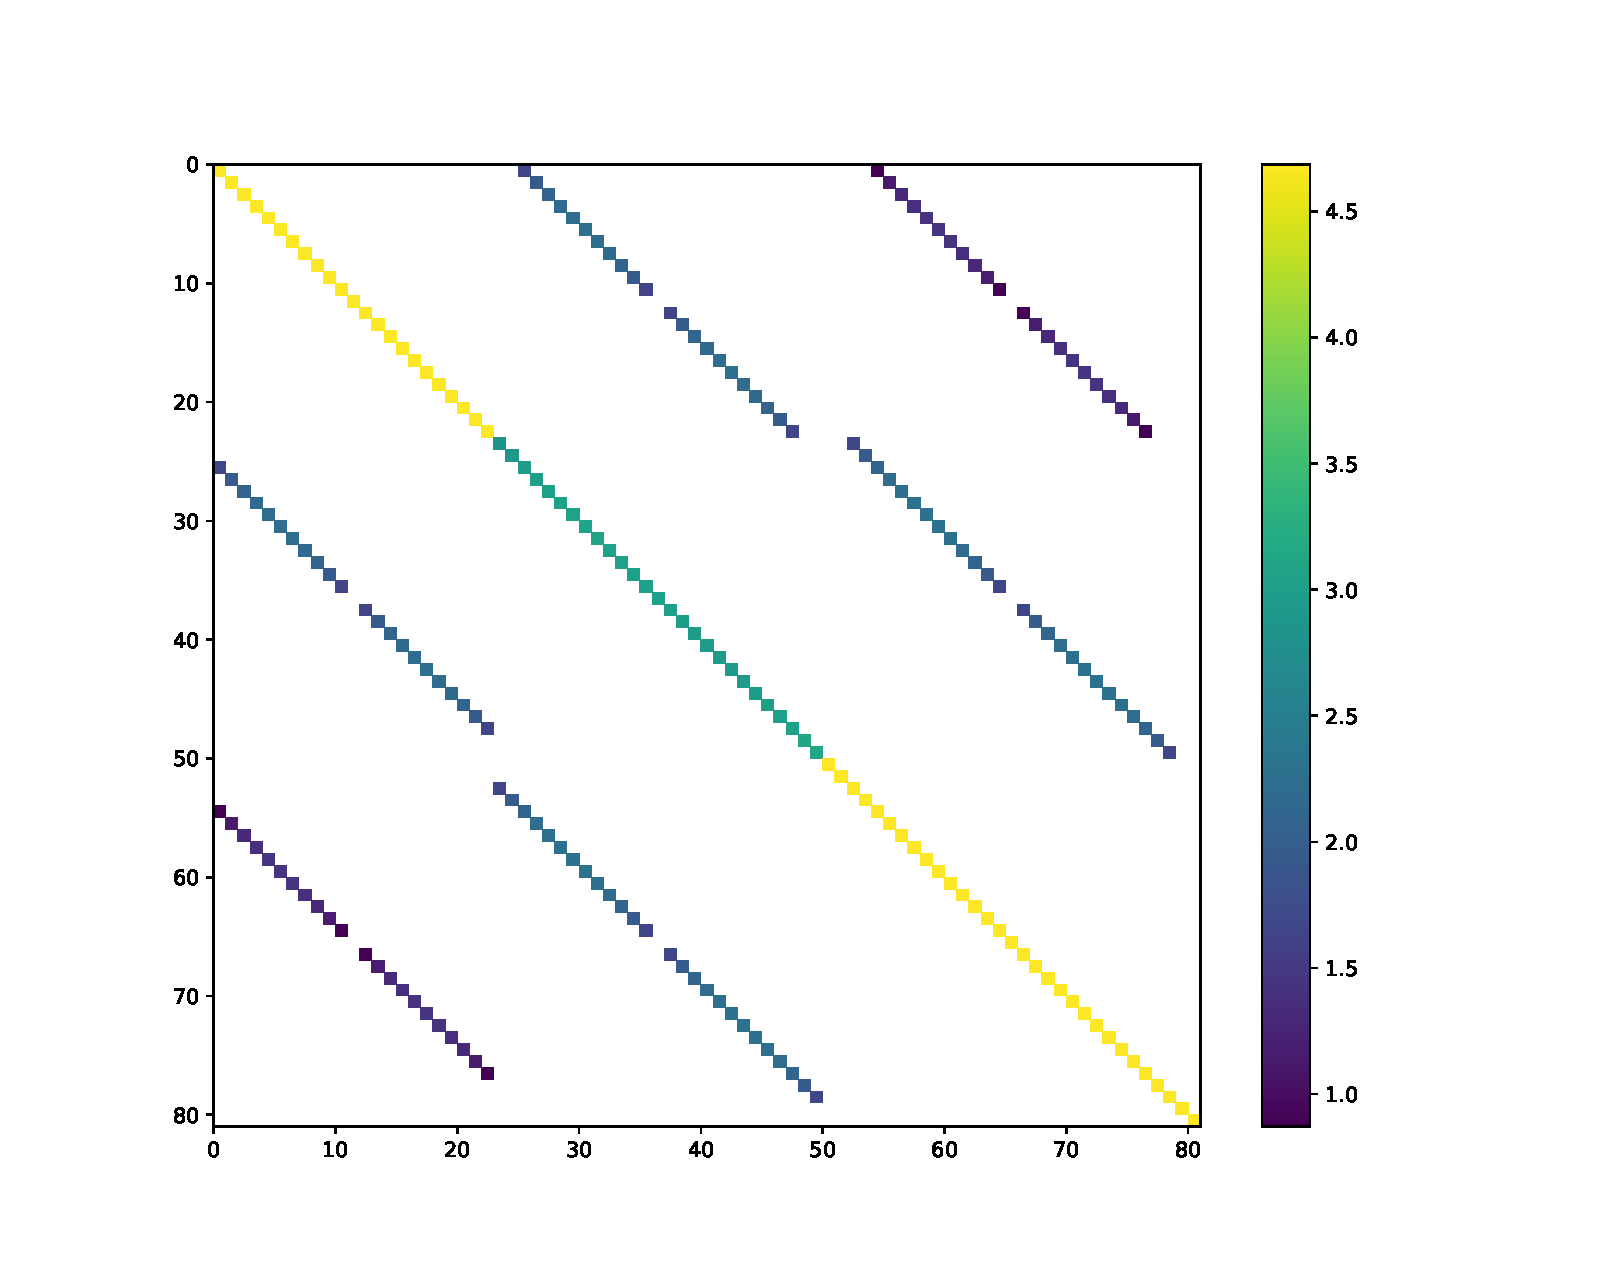
\includegraphics[scale=0.6,center]{Chapter2/figs/coup_mat}
\caption{Visualisation of $\log_{10}|Z_{k'k}|$ in $\mu Hz^2$ for the modes $\mode{0}{11}$, $\mode{0}{13}$, and $\mode{0}{15}$ with frequencies $603.69 \mu Hz$, $641.84\mu Hz$, and $677.55 \mu Hz$ respectively. White spaces correspond to $0$ value. Logarithm scale demonstrates the order of magnitude difference between self-coupling (diagonal elements), and cross-coupling (subdiagonal elements).Also notice that largest elements (yellow) are in the first and third section in the main diagonal. These are large because these frequencies are placed away from $\omref$ which is taken to be mean of the three mode frequencies. The relative weakness of the sub-diagonal terms compared to the main-diagonals is because $l-l'\geq 2$ forces $s\geq 2$ which makes the largest component of differential rotation, i.e. $w_1^0$, unable to couple these modes; $w_3^0$ and $w_5^0$ are one and two orders of magnitude smaller than $w_1^0$ respectively.}  
\label{fig:coup_mat}
\end{figure}